\section{Our findings}
\label{sec:our_finding}

\begin{figure}[!htbp]
    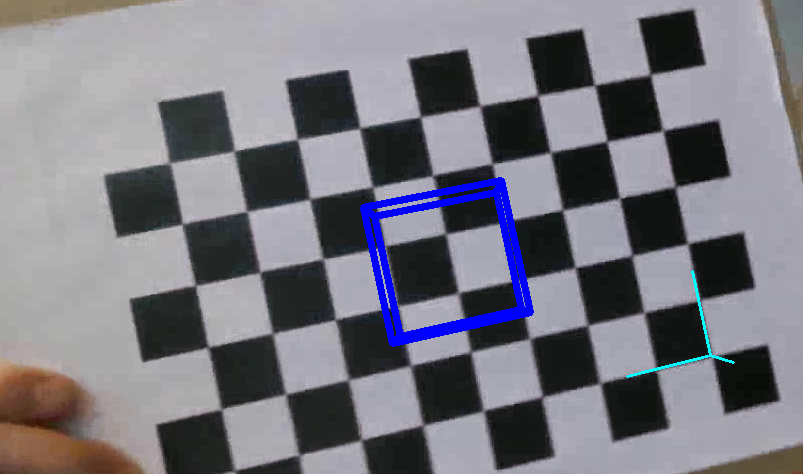
\includegraphics{pics/wireframe.png}
    \label{fig:wireframe}
    \caption{Wireframe of the augmented cube}
\end{figure}
In figure \ref{fig:wireframe} we see the first steps towards augmented reality.
It is kind of where we left off from assignment two, only with a new method. We
also implemented the same method as was used in assignment 2. This can be seen
in figure \ref{fig:wirefram_old}. This method give us a skewed result. Most
likely because of a bad homography. 

\begin{figure}[!htbp]
    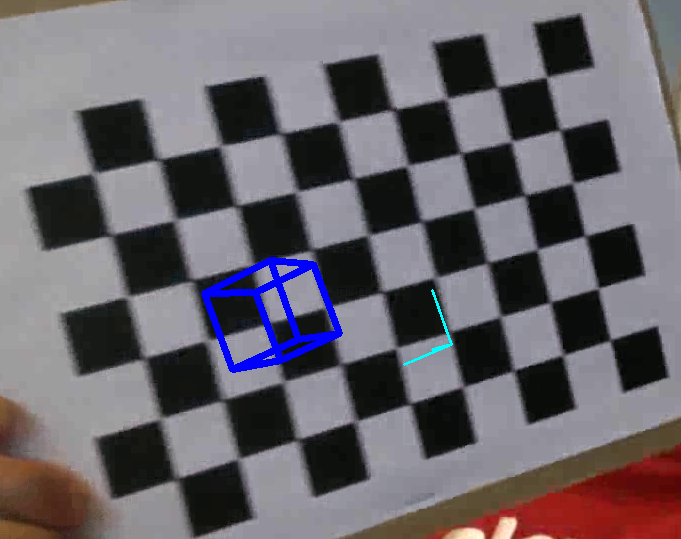
\includegraphics{pics/wireframeOld.png}
    \label{fig:wireframe}
    \caption{Wireframe of the augmented cube with old method}
\end{figure}

The difference between these two method is also clearly seen in \ref{fig:grid}
and \ref{fig:gridOld} respectively.  

\begin{figure}[[!htbp]
    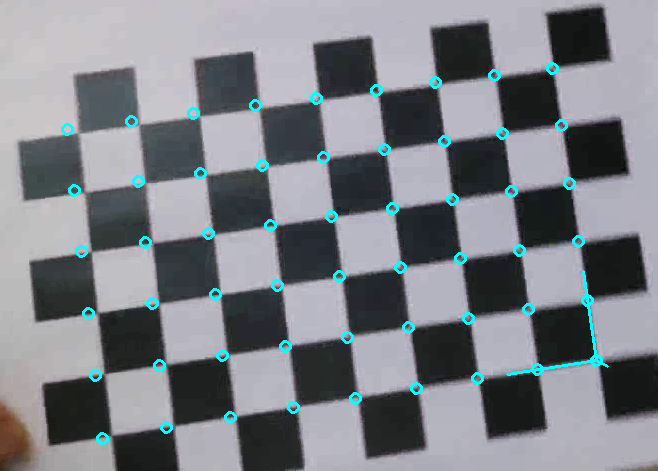
\includegraphics{pics/grid.png}
    \label{fig:grid}
    \caption{The augmented grid}
\end{figure}

\begin{figure}[!htbp]
    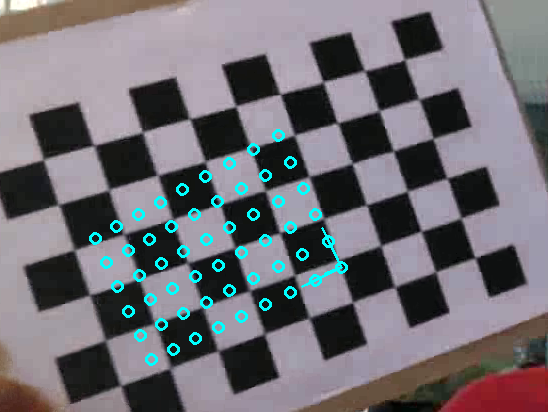
\includegraphics{pics/gridOld.png}
    \label{fig:gridOld}
    \caption{The augmented grid with the old method}
\end{figure}

Next up was adding textures to the cube to make it look cooler. The naive result
of this is seen in figure \ref{fig:noCulling}

\begin{figure}[!htbp]
    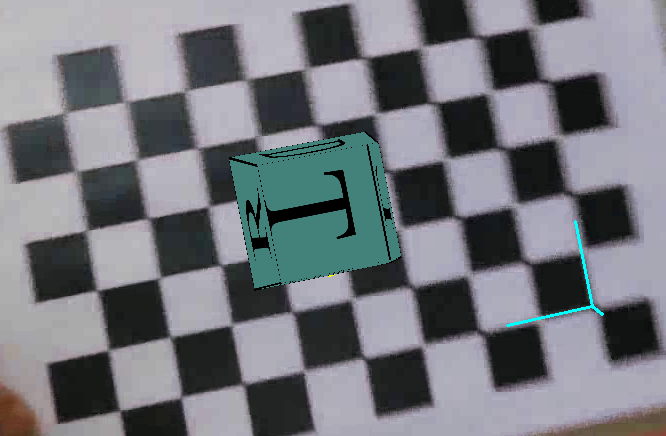
\includegraphics{pics/noCulling.png}
    \label{fig:noCulling}
    \caption{Naive texture mapping on cube}
\end{figure}


Obviously the approach used in figure \ref{fig:noCulling} is far from perfect
because all sides are visible. Even those that would be occluded by the cube
itself. This is fixed in figure \ref{fig:withCulling} where back-face culling
is applied to correctly hide the occluded faces

\begin{figure}[!htbp]
    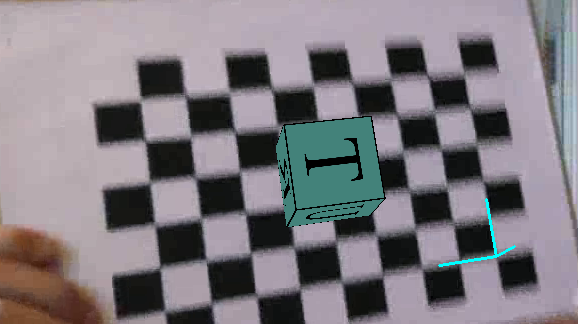
\includegraphics{pics/withCulling.png}
    \label{fig:withCulling}
    \caption{Texture mapping with backface culling on cube}
\end{figure}

The next part of the assignment focused on shading. The approach taken was 
based on the Phong illumination model and manipulates the RGB channels of the 
image on the cube face to give a shading effect. The first method implemented 
was flat shading. A successful result of this is seen in figure \ref{fig:flatShading}.

\begin{figure}[!htbp]
    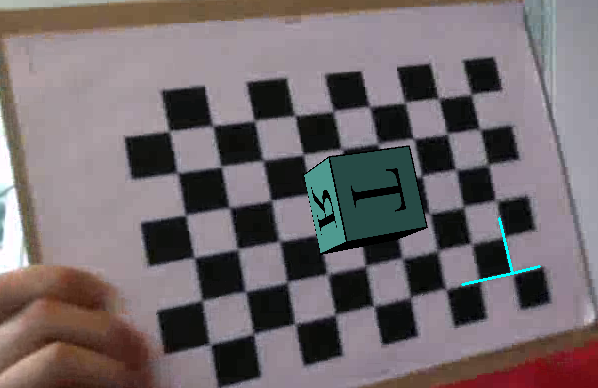
\includegraphics{pics/flat1.png}
    \label{fig:flatShading}
    \caption{flat shading on the figure}
\end{figure}

Here can be seen that the diffuse lighting hit's the top face more than the outward
facing face. Thereby leaving the outward facing darker. For illustrative purposes
figure \ref{flatRedAmbient} shows an example where the ambient lighting has a much
higher red value. What is seen is that the shadowy face (outwards facing) is more red 
than the face where the diffuse lighting falls. 

\begin{figure}[!htbp]
    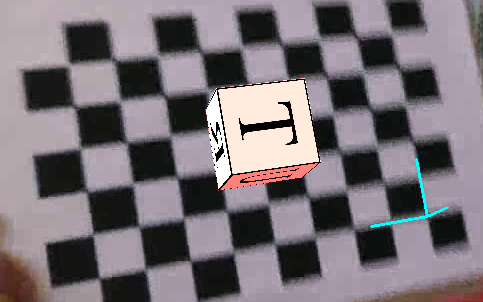
\includegraphics{pics/flatRedAmbient.png}
    \label{fig:flatRedAmbient}
    \caption{flat where the ambient value has it's red channel manipulated}
\end{figure}

The next shading method used is phong shading, which is more advanced and consequently 
more difficult to implement. An example of this is seen in \ref{fig:phongShading}. 
What can be observed is that the lighting falls more realisticly. Mainly because the light falls 
differently spread over the face. What can also be observed is that specular lighting has
a big effect on the quality of the results in figure \ref{fig:phongSpecularShadig}.
\begin{figure}[!htbp]
    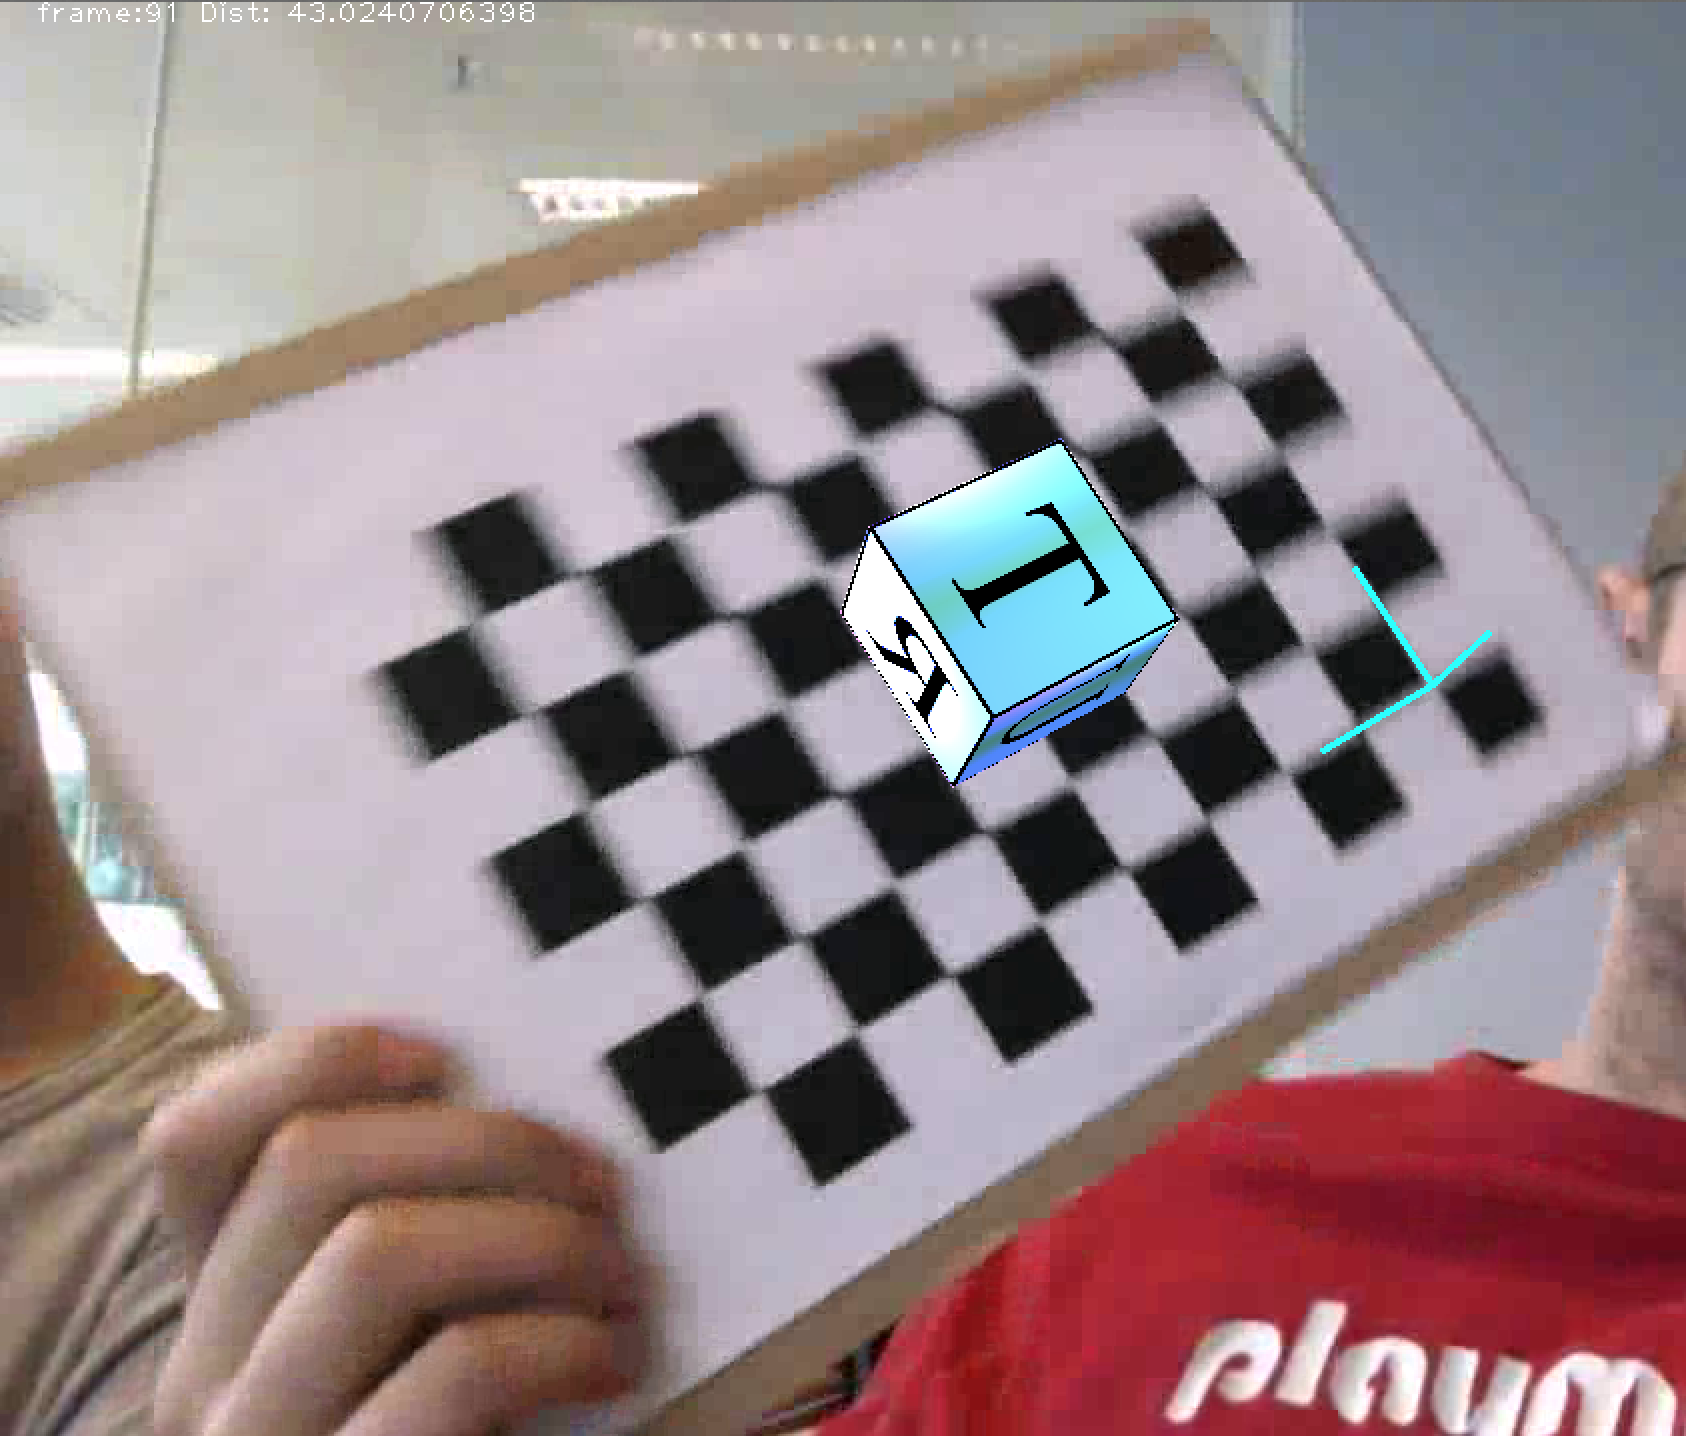
\includegraphics{pics/phongShading.png}
    \label{fig:phongShading}
    \caption{an example of Phong shading}
\end{figure}

\begin{figure}[!htbp]
    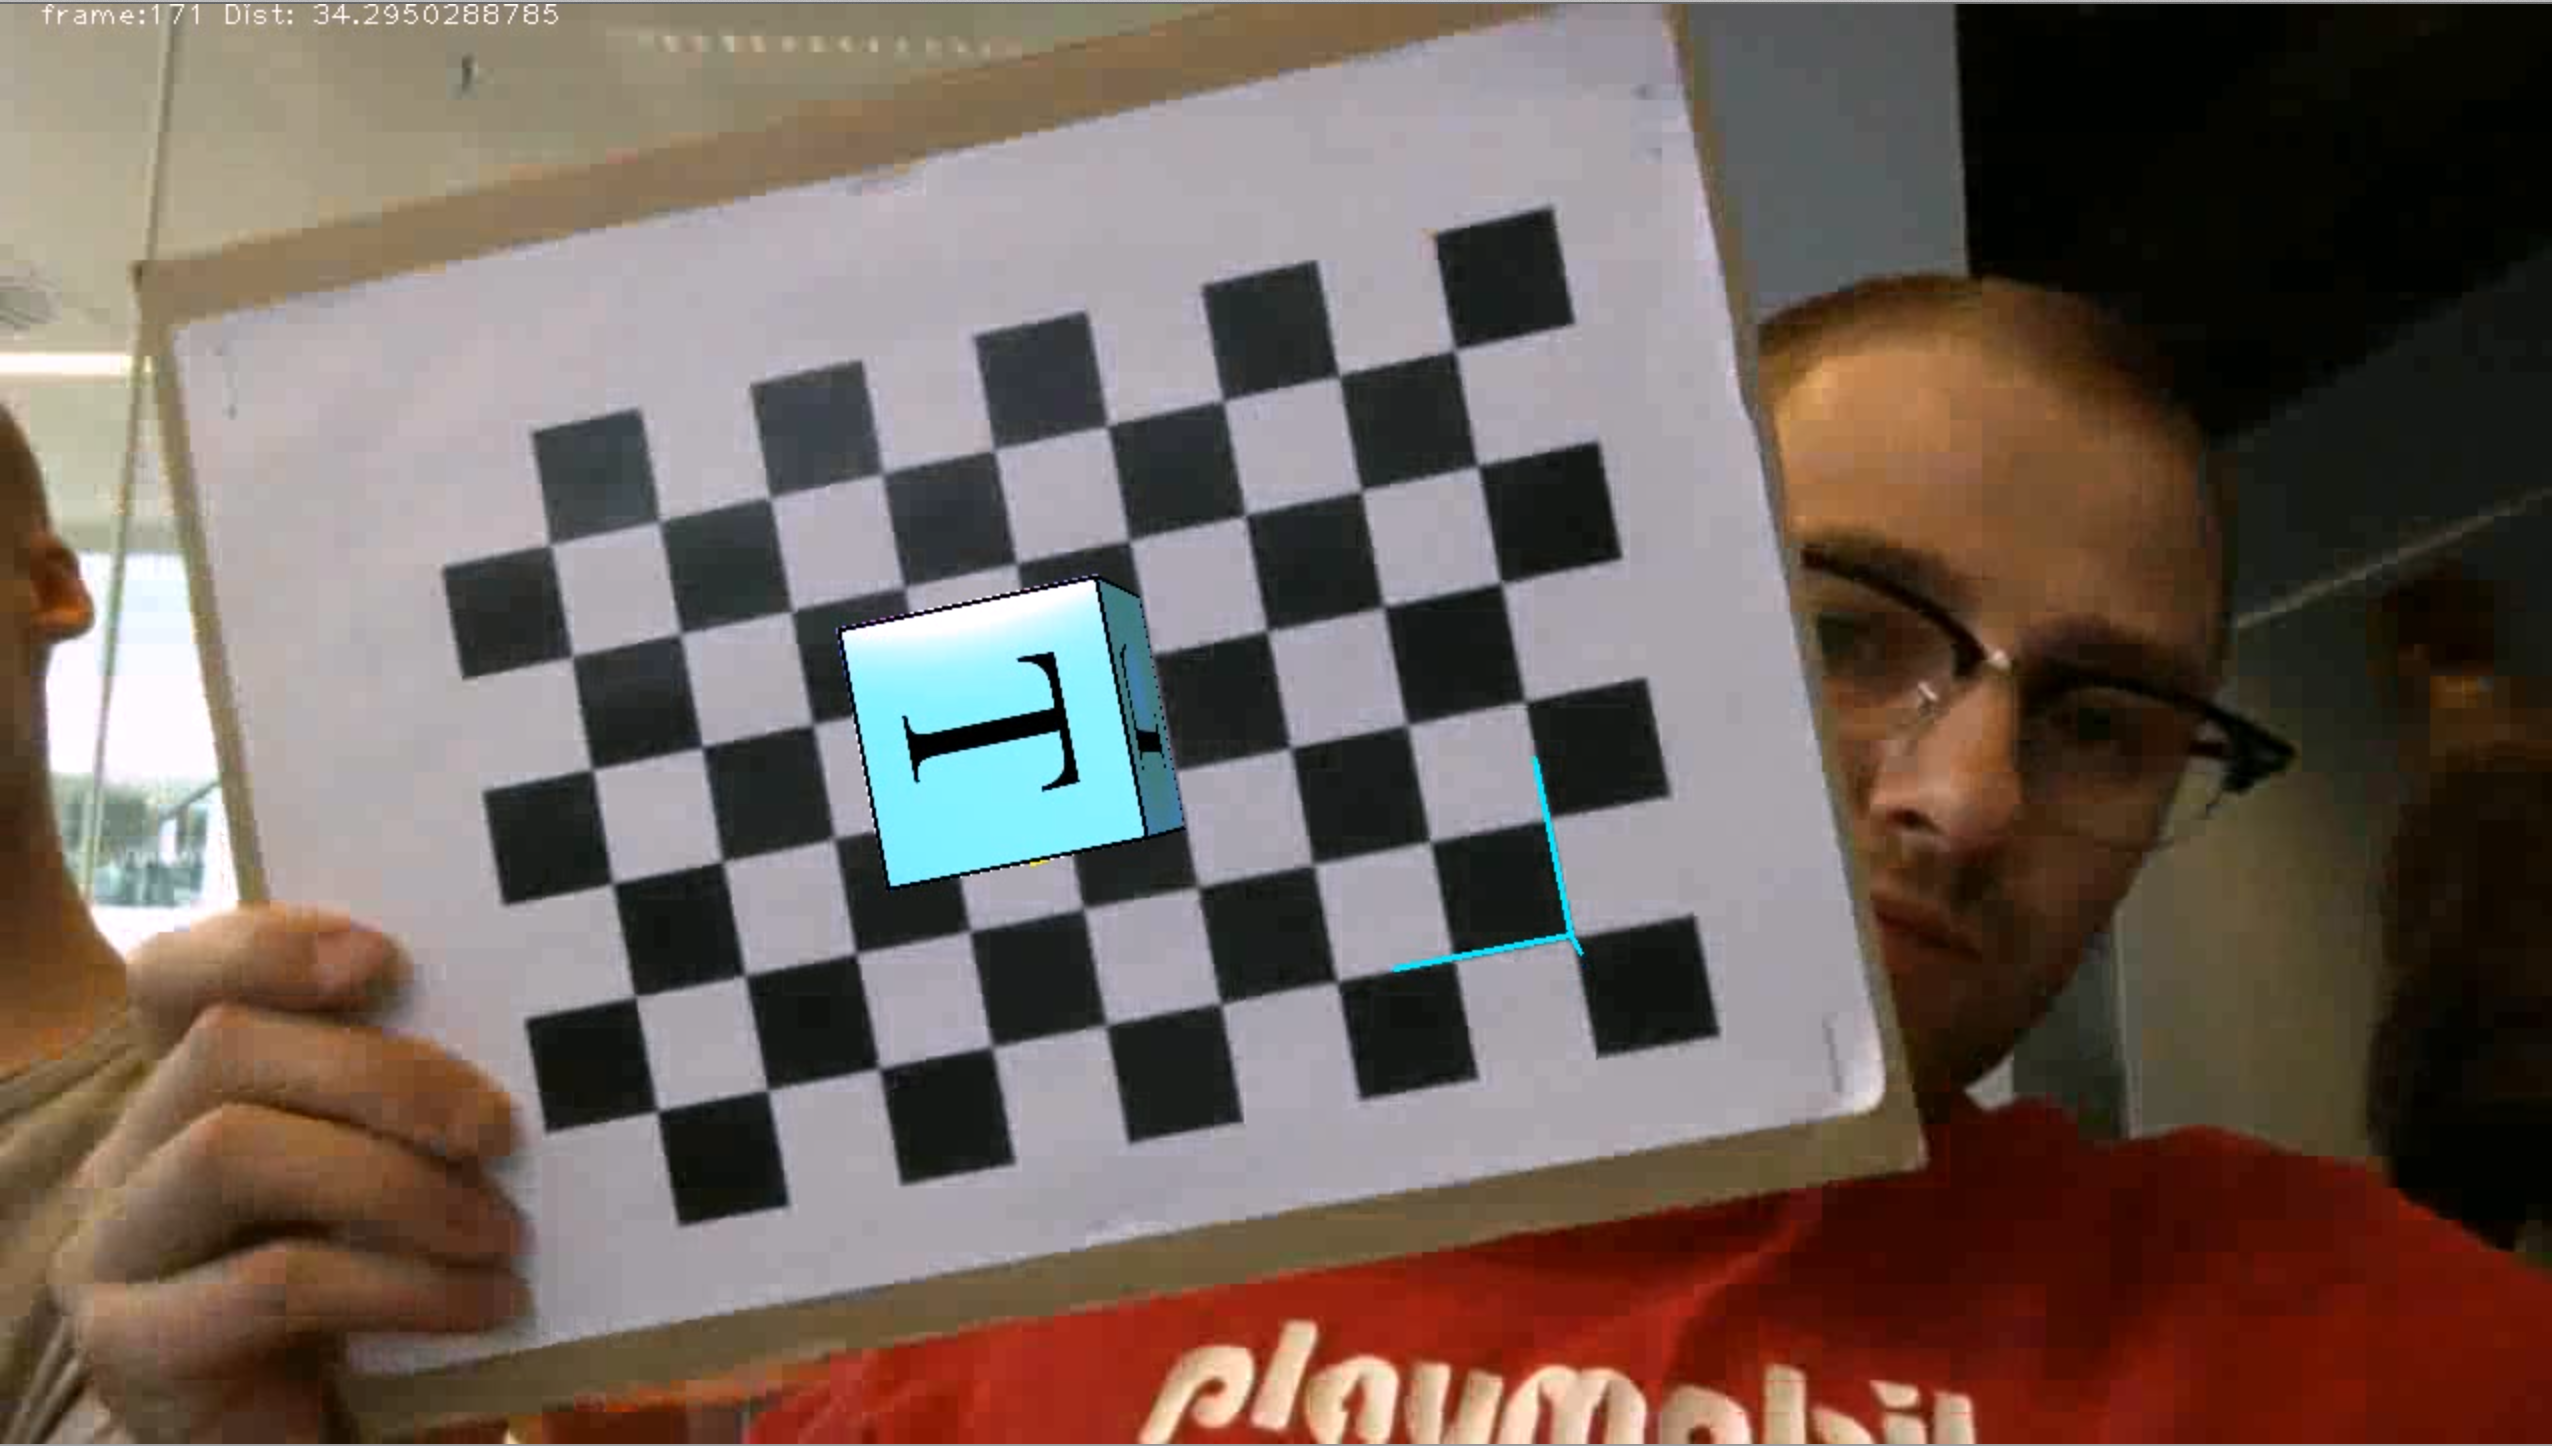
\includegraphics{pics/phongSpecularShading.png}
    \label{fig:phongSpecularShading}
    \caption{an example of Phong shading with the specular lighting having an impact}
\end{figure}
